\chapter{AirLogic} \label{ch:airlogic}
  \begin{figure}[h]
    \centering
    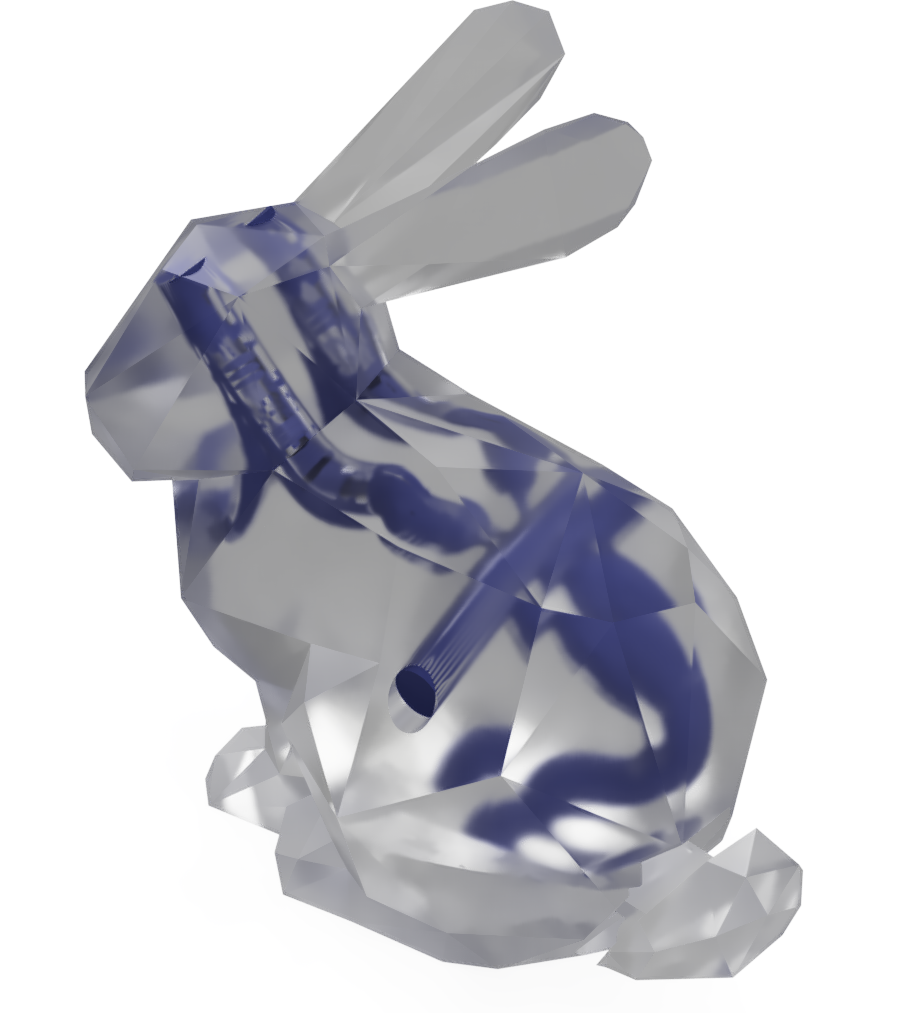
\includegraphics[width=0.33\textwidth]{print-and-play/airlogic/bunny-render.png}
  \end{figure}

  Despite the success of \at, \bh, and \mp in facilitating the construction of
  tangible devices that can sense, and provide output to user's interactions,
  they still require a computing device to process and identify the provided
  input, and to drive the output.  This limitation inspired me to think about
  the construction of tangible devices where \emph{everything} is encapsulated
  in the device: input sensing, logic processing, and output display. This
  upcoming chapter is the result of this exploration.

  This chapter, based on unpublished work~\cite{Tejada:}, introduces a toolkit
  for fabricating stand-alone tangible devices where all the input, logic
  processing, and output display are carried out in the device. In this chapter
  I present the set of air-powered widgets that make up the \al toolkit, and the
  underlying technologies that enable them. Additionally, and similarly to the
  previously discussed techniques, I developed a design environment to enable
  users to embed \al widgets into existing three-dimensional models. Last, this
  chapter closes with a set of illustrative applications, and discussions on
  \al's performance and possible directions for future work.

  The main challenge undertaken with \al was the design the widgets that
  comprise the toolkit. Arriving at the final designs for the logic widget
  entailed significant iterations, because of the limited documentation on the
  operation of these designs.


  \newpage

  This chapter is based on the collaborative effort described below.

  \vfill

  \noindent
  \textbf{Title}\\
  \textit{AirLogic: A Toolkit for 3D-printing Stand-Alone, Interactive Objects}

  \bigskip

  \noindent
  \textbf{Authors}\\
  \textit{\underline{Carlos E. Tejada}, Hyunyung Kim, Mengyu Zhong, Raf Ramakers, Daniel Ashbrook}

  \bigskip

  \noindent
  \textbf{DOI}\\
  \textit{In Manuscript.}

  \bigskip

  \noindent
  \textbf{Venue}\\
  \textit{--}

  \bigskip

  \noindent
  \textbf{What was the role of the PhD student in designing the study?}\\
  \textit{The PhD student was the first author of the paper, and responsible
    of the described studies.}

  \bigskip

  \noindent
  \textbf{How did the PhD student participate in data collection and/or development of theory?}\\
  \textit{The PhD student was responisble for study implementation, execution,
    data collection, and theory development.}

  \bigskip

  \noindent
  \textbf{Which part of the manuscript did the PhD student write or contribute to?}\\
  \textit{The PhD student contributed to all parts of the manuscript.}

  \bigskip

  \noindent
  \textbf{Did the PhD student read and comment on the final manuscript?}\\
  \textit{Yes.}

  \bigskip
  \vfill

  \newpage

  \subsubsection*{Abstract}
    The promise of on-demand fabrication of custom, interactive devices is
    closer to reality thanks to recent developments in 3D-printing of
    interactive devices. While recent work has presented novel ways to
    3D-print artifacts such as speakers, electromagnetic actuators, and
    hydraulic robots; these efforts are non-trivial to instantiate,
    requiring assembly of circuits or mechanical parts. The present work
    introduces \al: a toolkit for the creation of stand-alone, interactive
    objects using pneumatic widgets. Objects constructed using \al, require
    no electronic circuits, and little to no assembly of physical
    components. \al is comprised of a set of 12 pneumatic widgets, and a
    design environment, which designers can use to embed input, logic
    processing, and output capabilities to existing 3D models. We present
    an evaluation of the performance of our widgets, and a four
    applications that illustrate \al's potential.

  \section{Introduction}
    In recent years, digital fabrication research has broadened its
    focus from fabricating 3D shapes to creating
    functional and interactive objects, including
    speakers~\cite{Ishiguro:2014}, 
    electromagnetic actuators~\cite{Peng:2016}, and hydraulic
    robots~\cite{MacCurdy:2016}. While such objects offer useful
    functionality, the fabrication process is often laborious,
    requiring that end users modify object
    geometry~\cite{Ledo:2017}, assemble
    circuits~\cite{Murray-Smith:2008}, or 
    manually insert non-printable materials \cite{He:2017}. We
    envision a future where functional devices can be printed and
    instantly used, without the need for intervention during
    printing, post-print assembly, or training of machine learning
    models.

    As a step towards this vision, this paper presents \al, a novel
    technique to fabricate interactive 3D-printed devices that
    encapsulate all input, logic, and output as an integral part of
    the printed structure, and which are immediately usable once
    printed. \al accomplishes this by updating classic work in
    \textit{fluerics}\footnote{More commonly called
    \textit{fluidics}; we use \textit{fluerics} to avoid confusion
    with microfluidics.}~\cite{CharlesBelsterling:1971}, a nearly
    forgotten area of research that uses jets of air to perform
    computation without electricity or moving parts. While flueric
    technology was popular in the 70s
    it largely became obsolete with the advent of smaller, cheaper,
    and faster transistors. In this paper, we show how advances in
    additive manufacturing enable current generations of
    off-the-shelf fused-deposition modeling (FDM) printers to
    produce flueric input, output, and logic structures. In contrast
    to approaches requiring embedding non-printable material into 3D
    prints, \al's flueric structures are 3D printed as part of the
    object itself. As such, \al allows designers to prototype
    objects that are instantly interactive once 3D printed.
    
    This work contributes to the existing track of research on embedding
    functionality in objects during the fabrication process in order to
    facilitate and speed-up prototyping interactive
    devices~\cite{Valkeneers:2019, Ion:2017, Peng:2016}. \al
    is therefore a step in fulfilling the vision of fully 3D-printed
    interactive devices. This work contributes:

    \begin{enumerate}
      \item A set of 12 pneumatic widgets, consisting of input, output, and
        logic gates that can be fabricated using consumer-grade FDM
        3D-printers.
      \item A software plugin for Autodesk Fusion 360 that makes the
          pneumatic widgets available to users when designing
        \al objects.
      \item A technical evaluation to characterize the workings and
        performance of the pneumatic widgets.
      \item A set of example applications that illustrate \al's use
        in various scenarios.
    \end{enumerate}
    
  \section{\al Operating Principle}
    \al operates using pneumatics; however, unlike previous approaches
    which required complex fabrication techniques
    \cite{He:2017,Vazquez:2015,Slyper:2012} or were limited to sensing
    input points \cite{Tejada:2018, Tejada:2020}, \al uses a single-step
    fabrication process and senses a variety of input events, performs
    simple computations based on those events, and creates output based on
    the computations. The key principle is that---inspired in part by
    fluerics---we use 3D-printed geometry to enable a continuous flow of
    air to act as a \textit{power source}, allowing \al to perform
    functions analogous to those preformed by electrical circuits. Here we
    briefly explain how each of \al's three main parts (input, logic,
    output) work in the context of the sample object illustrated in
    Figure \ref{fig:app-bunny}, A; later sections describe these components in
    greater detail.

    After designing and printing the bunny, the user can immediately
    connect it to a pressurized air source using the single input channel
    embedded in the object. This air input is analogous to VIN or V+ in an
    electronic circuit. The air flows through channels and splitters
    fabricated in the body of the object (analogous to wires). The designer
    has specified two touch points on the bunny's surface. These are
    designed such that air vents to the atmosphere (analogous to ground) in
    the absence of touch. When blocked, however, the channels route the air
    to a flueric \texttt{OR} gate (described below). With either touch
    sensor covered, the air continues to flow to the oscillating actuator
    (very roughly analogous to a motor) embedded in the bunny's tail, which
    then wiggles up and down with the force of the air striking the paddle
    on its way to the atmosphere.

    While the functioning of the input and output widgets is fairly
    intuitive, the operation of flueric logic gates is less so.
    These operate on the principle of \textit{momentum transfer}
    between jets of air. The idea is that the course of an air jet
    can be changed by the force of another jet striking it from the
    side. In the case of the \texttt{OR} gate (schematically
    illustrated in Figure \ref{fig:logic-widgets}, B), a single jet proceeds
    directly at an angle through the central ``interaction area'' to the
    output. When both jets are present, they collide with each other,
    canceling each other's angle, and form a single coherent jet that exits
    the output. Of particular note are the vents to either side of the
    interaction area in the gate. While the same gate could be simply
    formed as a ``Y''-shaped pipe, any loading on the output (e.g. being
    blocked) would cause back-pressure throughout the system and impair the
    functionality of other components. The vents allow any such negative
    flow to be safely discharged to atmosphere.

  \section{Related Work}
    Our work touches upon multiple areas of research including the
    fabrication of interactive objects, fluidics, and analog computing.

      \subsection{Physical User Interface Toolkits}
        \al contributes a technique to fabricate stand-alone interactive
        objects using pneumatic principles to the field of physical user
        interface toolkits.

        Early efforts in physical user interface toolkits adopted a
        \emph{prefabricated} approach, where the different components of
        the toolkit are fabricated by a third-party, and end users
        assemble, but don't usually modify, them. One of the first efforts
        introducing physical user interface toolkits in the HCI literature
        is Phidgets~\cite{Greenberg:2001}. Its authors applied the concepts
        of Graphical User Interfaces (GUIs) widgets, to construct physical
        interaction controls using reusable components. Further iterations
        on this concept introduced connections between the
        components~\cite{Bdeir:2009}, novel
        form-factors~\cite{Hodges:2014}, or more powerful
        components~\cite{Villar:2012}. While prefabricating the different
        components of the toolkit reduces the design and assembly work for
        end users, they are limited to the component manufacturer's
        designs.
        
        To allow more customization, later endeavors resort to custom
        fabrication of their widgets and components. These efforts provide
        assistance to designers to construct custom widgets. Efforts like
        Midas~\cite{Savage:2012}, Pineal~\cite{Ledo:2017}, and
        PaperPulse~\cite{Ramakers:2015} enable users to construct widgets
        in order to fabricate interactive objects using custom touch
        sensors to wrap around existing objects, using ``remote widgets''
        on smartphones and watches, or fabricating predefined widgets using
        conductive inkjet printing. The main advantage of this approach is
        the increased flexibility it allows designers to
        include different types of widgets in different sizes,
        as needed. However, this increased flexibility comes at the cost of
        greater time and effort during the design process.

        \al draws inspiration from both types of physical user interface
        toolkits. We provide a set of predefined input, logic, and output
        widgets, which are customizable during the design stage, embedded
        in existing 3D models, and fabricated using commodity 3D printers.
        \al supports designers by providing a series of pre-validated
        widgets that can be re-used if desired, but that allow for enough
        customization to be used in a variety of applications.
        
      \subsection{Non-electrical computing systems}
        There is a long history in computing of non-electrical computation.
        The earliest computing devices, developed before the advent of
        electrical circuits, were mechanical: the earliest known
        computer, the Antikythera Mechanism (ca. 250--100
        BCE)~\cite{Efstathiou:2018}, was based on a complex system of
        gears, as was Babbage's proposed Analytical Engine
        (1837)~\cite{Bromley:1998}. Liquids were also used for
        pre-electronics computation of complex algebraic~\cite{Emch:1901}
        and differential~\cite{Moore:1936} equations.

        Despite the modern dominance of electronic computers, researchers
        have continued to explore alternative computing substrates, aiming
        to overcome limitations imposed by a reliance on electrical
        circuitry. Thorsen \etal developed complex microfluidic
        processors~\cite{Thorsen:2002} with application in biology and
        chemistry. However, fabricating such devices requires complex
        industrial processes, and—due to their "micro" nature—they operate
        at pressures and flow rates too low for actuating interactive
        devices~\cite{Thorsen:2002}. Aiming at robots composed entirely of
        soft components, Preston \etal created flexible pneumatic logic
        circuits based on kinking embedded soft tubes~\cite{Preston:2019b}.
        Although able to demonstrate AND, OR, and NOT operations,
        fabricating the gates necessitates a complex manual molding
        process, and incorporation into interactive objects requires
        assembly of both circuits and objects.
        
        Recently, Ion \etal demonstrated fully functional 3D-printed
        interactive digital devices comprised of metamaterial-based logic
        cells~\cite{Ion:2017}. Although theoretically capable of extending
        logical operations through any number of gates due to per-gate
        energy storage via a buckling mechanism, these devices must be
        manually reset after each use to recover the lost energy.

      \subsection{Fluerics}\label{sec:fluerics}
        Although many non-electrical computing systems have potential, none
        described in the preceding section are viable for achieving our
        goal of fabricating interactive devices requiring little to no user
        intervention in the production process. To do so, we require a
        computing substrate with the following properties:

        \begin{itemize}
          \item it should be able to be completely produced on a single
            printer with no user intervention;
          \item it should be capable of sensing, logic, and output;
          \item it should be embeddable in objects during printing;
          \item and it should be accessible to non-expert users.
        \end{itemize}
        
        The only available technology that meets all of these requirements
        is \textit{fluerics} or \textit{fluidic logic}, a nearly forgotten field
        started in the 1960s and active through the early 1980s.
        
        The basic principle underlying fluerics is simple: a constant stream
        of fluid moving in one direction can be deflected by the momentum
        of a second, less powerful, stream applied perpendicular to the
        first, by an amount proportional to the strength of the deflecting
        jet~\cite[p.~64]{CharlesBelsterling:1971}. By creating specific
        geometrical arrangements of channels that shape and direct the
        fluid streams, a multitude of operational elements can be
        created~\cite{Glaettli:1964}, as shown in Figure \ref{fig:logic-widgets}.
        
        Although fluerics was an active research area for nearly three
        decades, with widespread commercial application~\cite{:1968}, the
        majority of work in the space occurred before the popularization of
        interactive computing in the 80s (e.g.,~\cite{Foley:1984a}),
        limiting flueric interaction elements to simple
        buttons~\cite[p.~240]{:1968} and one-bit
        displays~\cite[p.698]{:1968}. Flueric technology was eventually
        eclipsed by the development of high-speed integrated electronics;
        today, the remaining research in fluerics largely concentrates on
        its potential for aerospace~\cite{Ferlauto:2017} or
        industrial~\cite{Lacarelle:2011} applications, leaving the
        potential for fluerics-based interactive devices largely
        unexplored.
        
        In order to make them as small and efficient as possible, fluidic
        logic devices were historically produced via chemical etching or
        machining, achieving channel sizes as small as
        0.5\,mm~\cite{Tanney:1970}. Such processes are inaccessible to end
        users. \al starts with basic flueric concepts and structures and
        updates and extends them to enable production on consumer-grade 3D
        printers. Using 3D printing allows us to achieve a high level of
        integration, incorporating flueric inputs, outputs, and logic gates
        directly into the structure of an object.

  \section{\al Widget Toolkit}
      To facilitate making \al interactive objects, we present a widget toolkit
      consisting of pneumatic structures for sensing input, for providing
      output, and for performing basic logic operations. All widgets have
      compatible characteristics and thus allow for interconnecting them to
      realize the desired interactive behavior. Below we describe the
      operational details of our 13 widget designs.
      
    \subsection{Input widgets}
      The internal design of our input widgets are based on an inverted
      T-joint as shown in Figure \ref{fig:input-widgets}, A. In its most
      basic design, pressurized air is injected on the left and will only
      continue its trajectory on the right side of the object when the air
      vent at the top is blocked.

      \begin{figure}
          \centering \includegraphics[width=0.8\columnwidth]
            {print-and-play/airlogic/InputOutputWidgets_v5.pdf}
          \caption{Our five input widgets. (A) Touch, (B) Button, (C),
            Switch, (D) Slider, (E) Dial.}
          \label{fig:input-widgets}
        \end{figure}

      \begin{enumerate}
        \item \emph{Touch}. 
          As shown in Figure \ref{fig:input-widgets}A, touch widgets use
          the most basic T-joint design, touching (or otherwise obstructing) the vent at the top
          allows the air to continue its trajectory inside the object.
        \item \emph{Push Button}. 
          Embedding a cap and slots inside the T-joint structure realizes a
          push button (Figure \ref{fig:input-widgets}, B). The cantilever spring
          design ensures the button cap always returns to its original
          position when released.
        \item \emph{Switch}. 
          Figure \ref{fig:input-widgets}, C shows the design of a switch.
          This widget design integrates a lever and a wedge on top of our
          basic T-joint structure. When moving the lever, the wedge
          covers the sensing structure, allowing the air flow to continue
          inside the object.
        \item \emph{Slider}.  
          Our slider widget consists in a series of our basic sensing
          structure connected in parallel to the air source in a straight
          line. On top of them, is a rail where a handle covers the sensing
          structures as it slides. We added stops at each sensing location
          to aid the user in finding them.
        \item \emph{Dial}.
          Similarly to the slider, the dial widget is comprised of a set of
          sensing structures, arranged in a circle. Atop these structures
          is a channel that guides a handle in circular motions. This
          handle has a structure in the bottom that covers our sensing
          structure once on top. The dial widget also contains stops at
          each of the sensing locations to allow the user to better find
          them.
      \end{enumerate}

      \subsection{Logic Widgets}
        Our logic widgets were inspired by classic works in fluid logic
        regarding jet deflection devices. Our widgets use the momentum of
        interacting jets of air to change the direction of the airflow in
        the system. These structures lend themselves to the implementation
        of logic functions (e.g., \texttt{AND, OR, XOR, NOT}) for their
        capability to modify the output of a system based on what inputs
        are present.

        While the majority of our input, and output widgets require
        moving parts in order to operate, our logic widgets are capable of
        computing digital logic operations by interacting jets of air (see
        Section \ref{sec:fluerics}). Our use of flueric structures to represent
        digital logic operations was motivated by their capability to carry
        out logic operations without any mechanical parts, or electronics.
        This capability highlights two main benefits. First,
        \emph{printability}. Because there is no mechanical or electronic
        parts to assemble, we are able to fabricate the main parts of an \al
        object as a single structure, requiring only the minimal assembly of
        external moving parts. Second, \emph{reliability}. The lack of moving
        parts means that the inner workings of the object will not degrade
        with use, with the added bonus that \al objects are particularly
        robust against movements and vibrations.

        Below we describe the operation of our four logic widgets.

        \begin{enumerate}
          \item \texttt{AND}. 
            We designed our \texttt{AND} logic gate widget
            (Figure \ref{fig:logic-widgets}-A,1) inspired by classic works in
            flueric jet deflection devices. This design presents our input
            controls to the left, and a single output on the middle right,
            with vents at the top and bottom. When only a single input is
            present (Figure \ref{fig:logic-widgets}-A,2), the flow is directed to
            the respective vent channel. If both inputs are present,
            however, their corresponding jets collide, redirecting the flow
            to the output channel (Figure \ref{fig:logic-widgets}-A,3).

          \item \texttt{OR}. 
            Our \texttt{OR} logic gate widget
            (Figure \ref{fig:logic-widgets}-B,1) is also based on classic works
            in fluerics. This design is made up of two inputs channel in
            the left, an output channel to the right, and two vents in the
            top and bottom. This design operates as an ``inclusive or'',
            meaning that if any of the inputs are active
            (Figure \ref{fig:logic-widgets}-B,2), the flow is directed to the
            output channel. Additionally, when both inputs are active, the
            flow from each combines and the resulting jet is directed to
            the output channel.

          \item \texttt{XOR}. 
            In order to implement our exclusive or (\texttt{XOR}) logic
            gate widget, we make use of the same design previously
            discussed for our \texttt{AND} logic gate, varying the location
            of the output and vents. In this configuration, the output
            channels are located in the top, and bottom right, while the
            input remain unchanged from the \texttt{AND} design. When a
            single input is present, the air jet is directed to the
            respective output vents (Figure \ref{fig:logic-widgets}-C,1). If both
            inputs are present, however, their respective jets collide,
            redirecting the flow to the center vent
            (Figure \ref{fig:logic-widgets}-C,2).

          \item \texttt{NOT}. 
            Last, our \texttt{NOT} logic gate widget, we likewise utilize
            the same design previously discussed for our \texttt{AND} and
            \texttt{XOR} logic widgets, with some changes on the location
            of output and vents. When employed as a \texttt{NOT} logic gate
            widget, this design presents an input and a power channel on
            the left, and an output in the lower right with two vents above
            it (Figure \ref{fig:logic-widgets}-D,1). In this configuration the power
            channel provides a constant flow of air, which is directed at
            the output channel (Figure \ref{fig:logic-widgets}-D,2). If there's flow
            incoming from the input channel, this jet collides with the
            power jet, causing the flow to be redirected to a vent
            (Figure \ref{fig:logic-widgets}-D,3).
        \end{enumerate}
        
        \begin{figure}
          \centering
          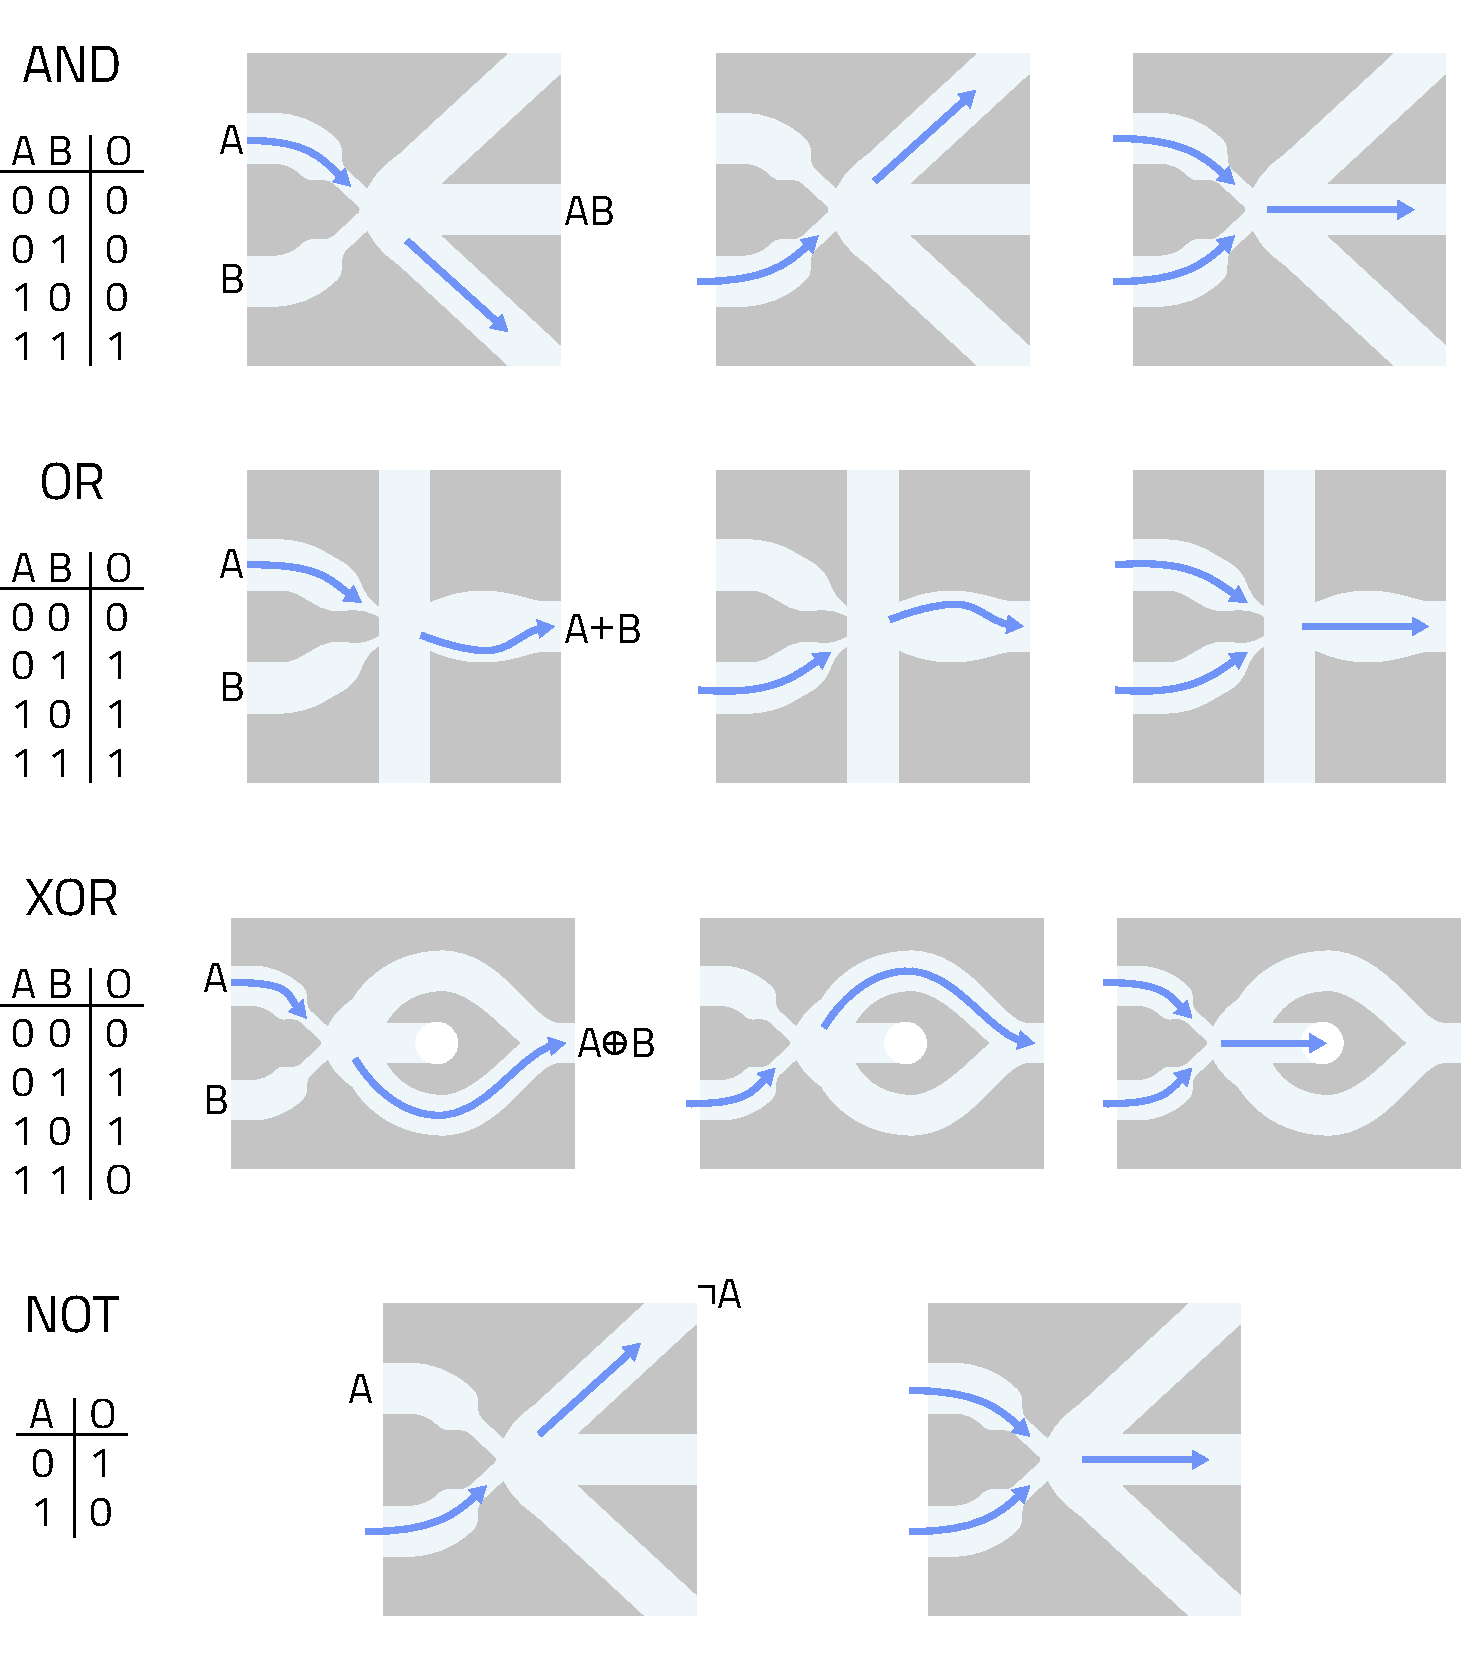
\includegraphics[width=0.8\textwidth]
            {print-and-play/airlogic/LogicGates_v2.pdf}
          \caption{AirLogic logic widgets. (A) \texttt{AND}, (B)
            \texttt{OR}, (C) \texttt{XOR}, (A) \texttt{NOT}.}
        \label{fig:logic-widgets}
        \end{figure}

      \subsection{Output Widgets}
        We were interested in displaying output in as many modalities as
        possible. We developed different air powered widgets that can
        present acoustic, visual and vibrotactile output as the result of
        the logic operations carried out by our logic widgets.

        \begin{enumerate}
          \item \emph{Pin}. 
            Inspired by research in shape-changing
            interfaces~\cite{Follmer:2013}, we designed our pin widget to
            provide visual output as a result of our logic operations
            (Figure \ref{fig:output-widgets}-A). Our pin widget is comprised of a
            cylindrical piston inside a camber. This piston can be actuated
            using compressed air, reaching a height of up to 4\,cm.
          \item \emph{Whistle}. 
            Our whistle widget (Figure \ref{fig:output-widgets}-B) is used to
            provide acoustic output as a result of a logic operation. This
            widget is made up of three main components: an intake, a
            fipple, and a chamber. Air resulting from our logic operations
            enters the whistle widget through the intake, and exhausts
            through the fipple, making a tone while doing so. By varying
            the size of the internal chamber in our whistle, we can change
            the tone generated~\cite{Helmholtz:1885vp}.
          \item \emph{Oscillating actuator}. 
            Another manner to provide visual output is to agitate sections
            of an \al object. To do so, we constructed a wiggler widget
            (Figure \ref{fig:output-widgets}-C), comprised of a lever that is
            pushed by incoming jets of air. When moving, the lever shortly
            falls out of phase with the air jet, and returns to its original
            position, causing it to be pushed once more.
          \item \emph{Vibration motor}. 
            In order to provide vibrotactile feedback on an \al object, we
            designed a vibration motor widget
            (Figure \ref{fig:output-widgets}-D). This widget operates similarly
            to electronic vibration motors commonly found on smartphones,
            where a mass is spun up to create different vibration patterns.
            In our design, air incoming from our logic widgets spins a
            fan-like structure, causing vibrations in the \al object.
        \end{enumerate}

        \begin{figure}
          \centering
          \includegraphics[width=0.8\textwidth]
            {print-and-play/airlogic/Widget_Output.pdf}
          \caption{Output widgets. (A) Pin, (B) whistle, (C) oscillating
            actuator, (4) Vibration Motor}
          \label{fig:output-widgets}
        \end{figure}

  \section{Designing \al Objects}
    \al offers two strategies for designing interactive objects: a
    prototyping workflow that allows for rapid testing, and a design
    pipeline for embedding \al widgets inside existing 3D models.

    When prototyping the desired interaction, the designer can construct a
    transit using our encapsulated widgets. These widgets can be connected using
    off-the-shelf 6\,mm wide plastic tubing, and powered by a constant air
    source. Once the design is completed, it can be translated to an existing 3D
    model.

    Further, to aid designers augment their 3D models with \al
    functionalities, we developed a widget library, available as a plugin
    for Autodesk Fusion 360, shown in Figure \ref{fig:design-environment}. Our
    library contains instantiated versions of all of our widgets, enabling
    the designer to embed input, logic processing, and output capabilities
    to existing 3D models in a single step. The design process starts by
    importing an existing geometry into the CAD software. Once loaded, the
    designer selects the desired input, logic and output widgets to use.
    Last, using an algorithm similar to PipeDream~\cite{Savage:2014}, we create
    channels connecting the widgets.

    While prototyping with encapsulated widgets is a heavily manual process for
    the designer and involves making many connections, fabricating and
    assembling an \al-powered 3D model with internal widgets requires little
    intervention. The majority of the object is printed as a single structure,
    involving only the assembly of moving parts (e.g., button, slider), and
    aesthetic covers.

    \begin{figure}
      \centering
      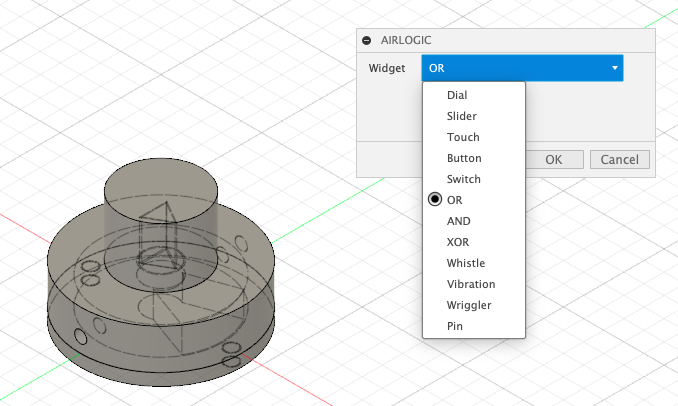
\includegraphics[width=0.8\textwidth]
        {print-and-play/airlogic/Design Environment.png}
      \caption{The widget library (right) and a Dial widget dropped by
        using the interface. In the interface, users can choose widgets and
        insert them into their design.}
      \label{fig:design-environment}
    \end{figure}

  \section{Implementation}
    Our logic widget designs are comprised of three main components: two
    input channels, an interaction area, and output channels and vents. We
    systematically explored the effect of each of these components by
    individually varying them while recording the barometric response of
    our designs. We found that using input, and output channels 2\,mm, and
    5\,mm in width gave us the best trade-off between performance, and
    pressure output to further drive our widgets. In order to avoid
    unnecessary changes in pressure within our system, we use 5\,mm
    channels to chain our widgets together.

    In order to make our approach accessible to a broader audience, we
    chose to implement \al using consumer-grade 3D-printing hardware. We
    constructed our test and prototype objects using both FDM and SLA
    technologies: an Ultimaker S3, a Creality Ender 3 Pro, and a Formlabs
    Form 2. During our tests, we discovered that the printing layers can cause
    unwanted turbulence when air flows through our air channels, negatively
    affecting the performance of our designs. We mitigate this issue by
    fabricating our prototypes using a minimum layer height of 0.03\,mm. 

    In addition to focusing our efforts to enable \al with consumer-grade
    3D-printing equipment, we also designed \al to be implemented using
    single-material printers. While this allow us to reach a broader
    audience, it came at the cost of very minimal assembly of moving parts.
    Multi-material printers can construct \al objects as a single structure
    by embedding dissolvable, or breakable support materials, however \al
    objects constructed with single material printers must have their widgets
    with moving parts (e.g., buttons, sliders, vibration motors) printed
    separately and manually assembled.

    We constructed an experimental setup to test our \al prototype designs.
    This setup was comprised of JunAir 2000-40PD air compressor, and Festo
    MS4-LR-1/4-D5-AS valve.

  \section{Validation}
    To validate \al and assess its practical feasibility, we empirically
    evaluated our widgets' capabilities to fabricate stand-alone
    interactive objects, and developed four illustrative applications.

    \subsection{Technical Evaluation}
      In order to understand \al's capabilities to fabricate stand-alone
      interactive devices, we empirically evaluated our widgets. We wish to
      understand the barometric pressure requirements of our designs, and
      how they can connect to each other. We recorded the barometric
      pressure responses of our designs by measuring the relation between
      the barometric pressure provided to our designs with the barometric
      pressure they discharge. We repeated this measure for 5 distinct
      input pressures, for all of our widgets, while noting if the widgets
      were working as expected.
      
      This experiment enables us to understand two main qualities of our
      designs. First, it allows us to understand the operating pressure
      ranges for our designs by identifying the pressures where our widgets
      perform bests. Second, it informs the pressure needs of our designs
      by establishing the losses in barometric pressures to be expected in
      our designs.
      
      To carry out our evaluations we constructed an evaluating setup
      consisting of a JunAir 2000-40PD air compressor, a Festo
      MS4-LR-1/4-D5-AS valve, an analog Panasonic PS-A (ADP5) barometric
      sensor. We printed encapsulated versions of our widgets, and
      connected their output channels to our barometric pressure sensor
      using off-the-shelf rubber tubes.

      \subsubsection{Results}
        Our tests uncovered that the operating pressures of our widgets
        vary with their type. Our input widgets perform best when powered
        with a constant air source with pressures from 50 kilopascals (kPa), to
        200 kPa. In contrast, our logic widgets presented an operating range of
        50 to 300 kPa, while our output widgets operate best when
        actuated with pressured from 150 to 250 kPa. 

        In addition, we found that, in average, our logic widgets lose half of
        the input pressure when processing their respective operations, while
        our input widgets designs present a neglible pressure loss. We did not
        evaluate the pressure losses of our output widgets, as they are intended
        to be the last element in our designs. A detailed view of our results
        can be found in Figure \ref{fig:pressure-losses}.

        \begin{figure}
          \centering
          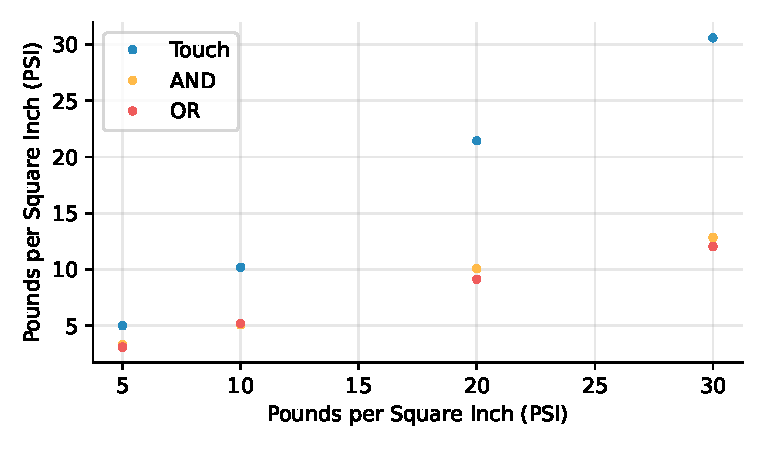
\includegraphics[width=\textwidth] {print-and-play/airlogic/pressure-losses}
          \caption{Pressure losses}
          \label{fig:pressure-losses}
        \end{figure}

    % Expand descriptions
    \subsection{Example Applications}
      In this section we present a series of applications constructed using
      \al. These applications illustrate \al's capabilities and potential
      for fabricating stand-alone, custom interactive objects without the
      use of any electronics.

      \subsubsection{Interactive bunny}
        Using our touch, \texttt{OR}, and wiggler widgets, we constructed
        an interactive bunny that wiggles its tail when pet in the
        correct locations.

        \begin{figure}[h]
          \centering
          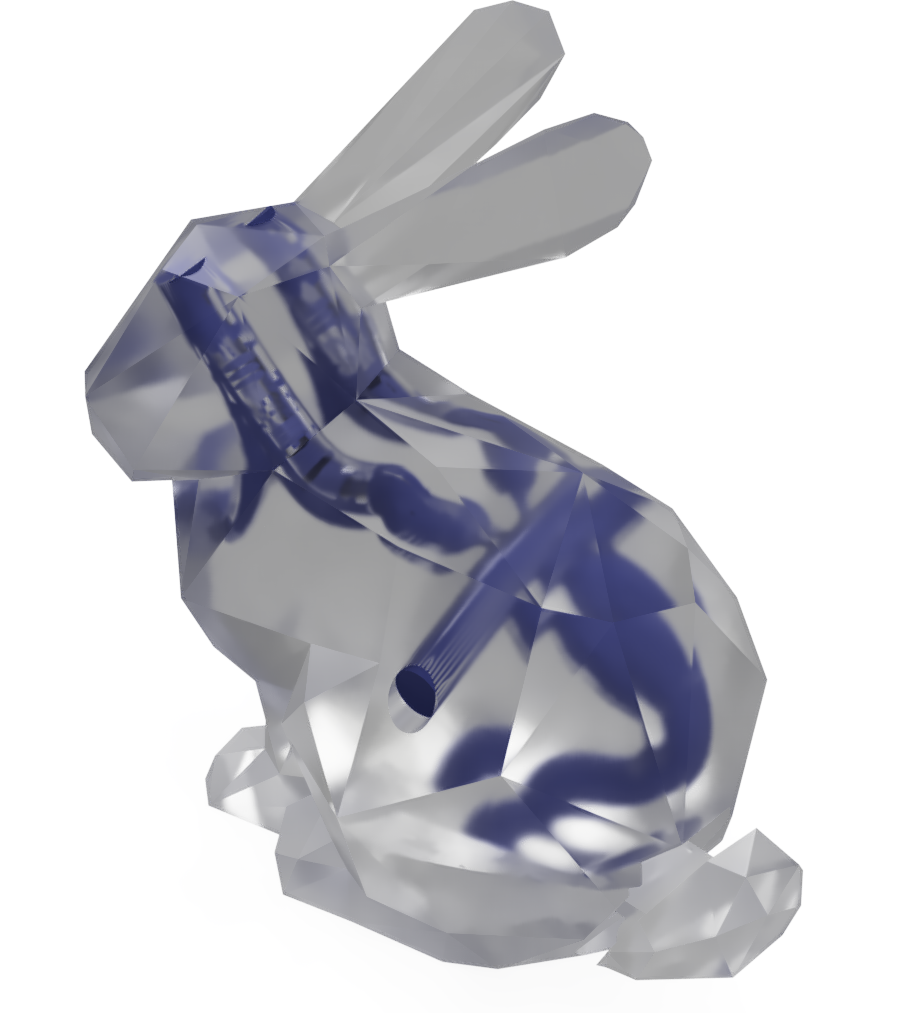
\includegraphics[width=0.7\textwidth]{print-and-play/airlogic/bunny-render.png}
          \caption{Interactive bunny}
          \label{fig:app-bunny}
        \end{figure}
      
      \subsubsection{Pitch switch}
        \label{sec:pitch}
        We used our slider, button, \texttt{AND}, and whistle widgets to
        fabricate a pitch selector. The user selects the frequency she wants to
        play using a slider, and when the ``play'' button is pressed, the
        desired tone is played using the respective whistle.

        \begin{figure}[h]
          \centering
          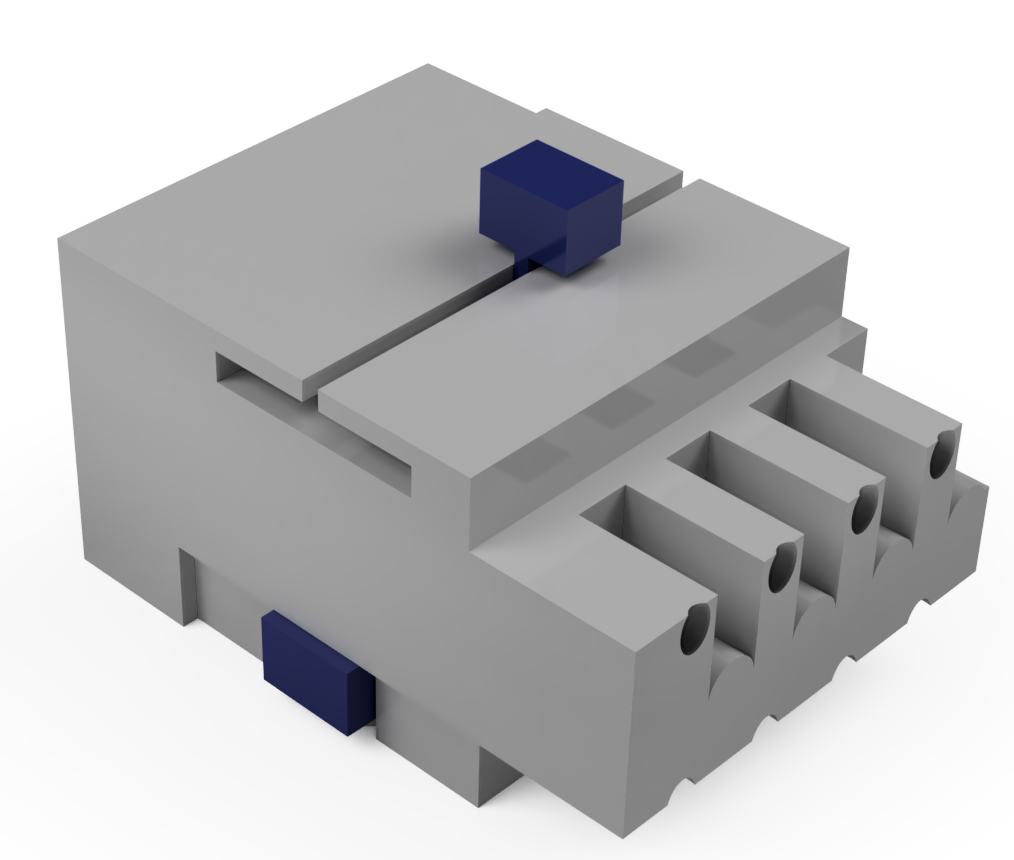
\includegraphics[width=0.7\textwidth]{print-and-play/airlogic/whistle-render.png}
          \caption{Pitch slider}
          \label{fig:app-slider}
        \end{figure}
      
      \subsubsection{Interactive puzzle}
        \label{sec:puzzle}
        By modifying our button widget, we constructed an interactive
        puzzle using the letters U, I, S, and T. When arranged in the
        correct order to spell UIST, a pin with a flag attached is raised.

        \begin{figure}[h]
          \centering
          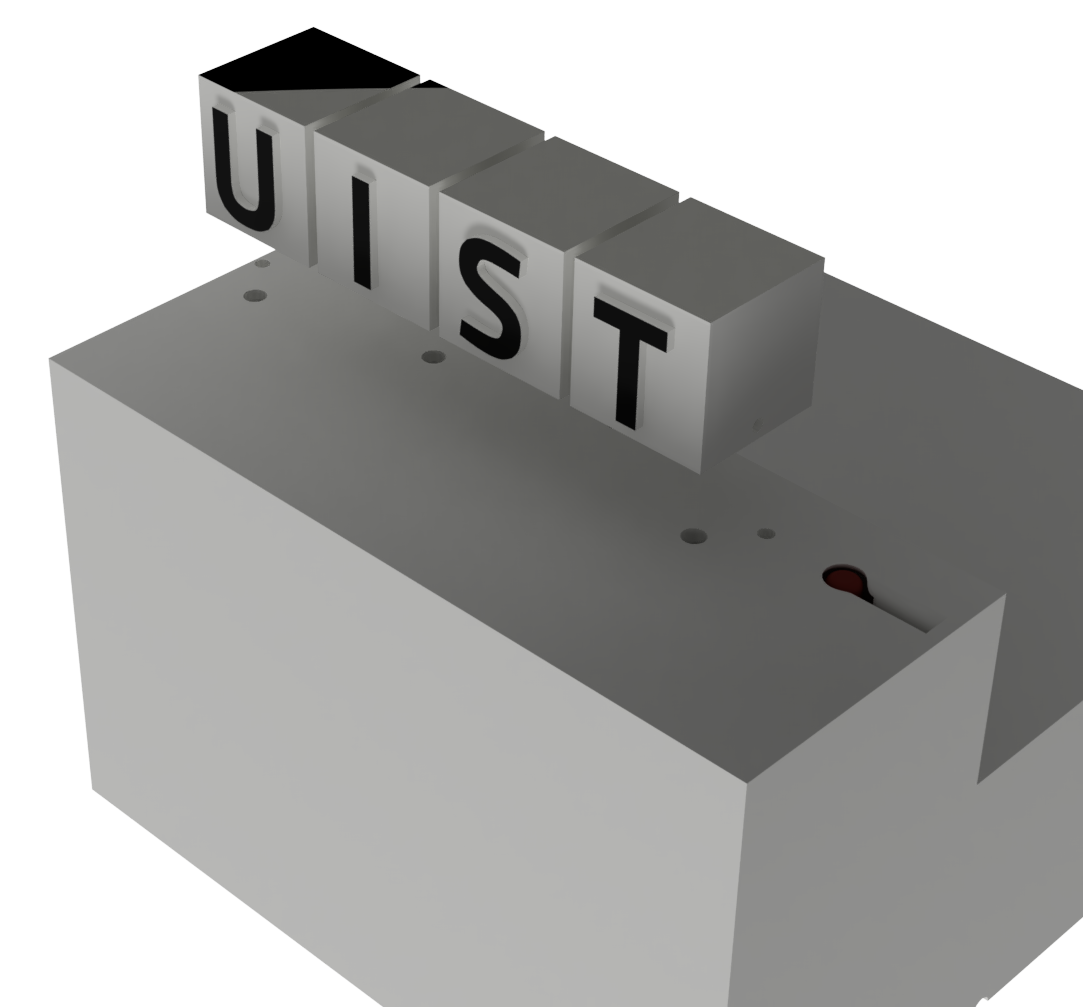
\includegraphics[width=0.7\textwidth]{print-and-play/airlogic/puzzle-render.png}
          \caption{Interactive Puzzle}
          \label{fig:app-slider}
        \end{figure}
      
  \section{Discussion \& Limitations}
      \subsection{Chaining logic widgets}
        While our applications illustrate the capacity of using multiple
        logic widgets in an \al object (see Figure \ref{sec:pitch} and
        Section \ref{sec:puzzle}), this functionality is limited in our current
        implementation. During exploratory tests we found that our logic
        widget designs could be connected three different ways: in
        parallel, balanced chained \texttt{AND}, and chained \texttt{OR}. We are
        not able to support unbalanced chained \texttt{AND}, and combinations.

        The paramount reason that we can't do these things is that our
        \texttt{AND} design is reliant on identical pressures on both input
        channels in order to function correctly. If one channel has more
        pressure, and therefore more momentum, than the other, it pushes
        the jet towards the top-right channel, rather than the middle
        right. This means that, if an \texttt{AND} widget were to be
        connected after an \texttt{OR}, which can be activated using one or
        two inputs, we would have to dynamically regulate the pressure of
        the second input for our \texttt{AND} widget depending on the
        number of inputs used in the previous \texttt{OR} widget.

        In future iterations of this work we aim to tackle this issue by
        standardizing the output from our logic widgets. Doing so will
        guarantee that the results from our logic operations will have the
        same pressure profile than our input widgets, no matter how many
        inputs are used to actuate them. To achieve this, we will explore
        two avenues. First we will research the use of active fluidic
        designs to construct our logic widgets. Our current designs are
        based on passive fluidic logic devices, where the the operation is
        performed using flow coming from the inputs. Using active designs, which
        contain a continuous air jet inputs interact with, will mean that the
        output barometric pressure for our widgets is always the same: that of
        the power air jet. Second, we will explore the use of fluidic
        amplifiers~\cite{CharlesBelsterling:1971}.  These structures increase
        the velocity of an incomming jet of air by switching an existing,
        constant jet from one outlet to another.
        
      \subsection{Exploring different fabrication methods.} 
        During our explorations we constructed our widgets using both FDM
        and SLA printers. Interestingly, despite their higher resolution of
        25 microns, widgets fabricated using SLA printers performed worse
        than those constructed with FDM ones. We suspect this is due to the
        fabrication pipeline of SLA printers where the resulting object
        needs to be washed before it is cured. If some resin deposits remain in
        our air channels after the wash, they will turn into partial
        blockages once cured. These blockages, given the small size of our
        channels, and high pressure sensitivity of our designs, can
        adversely affect our performance. To validate this theory, we
        fabricated a single \texttt{AND}, and washed it using fresh
        isopropyl alcohol, obtaining promising results, however, more
        experimentation is still needed.

        Additionally, we wish to explore subtractive fabrication methods for
        constructing our widgets. We believe that because of its high precision
        and clean cuts, laser cutting equipment presents a promising alternative
        to fabricate \al objects. While \al objects constructed using laser
        cutting equipment would require significantly more manual assembly than
        our current implementation and would likely be limited to 2D, we
        envision a further iteration of our design environment to provide
        stencils and assembly guides for \al designs fabricated on such
        machinery.
        
      \subsection{Comparison with electronics}
        Despite the potential interactions that \al enables designers to
        embed into 3D-printed objects, it falls short of what can be
        enabled using off-the-shelf electronic toolkits such as
        Arduino~\footnote{\url{https://www.arduino.cc/}}. While electronic
        toolkits allow for greater flexibility and variety of interactions,
        it comes at the cost of complex assemblies. In order to create an
        interactive device using an off-the-shelf electronic toolkit, the
        designer must posses engineering expertise in order to chose the
        correct components, assemble them into a working circuit, and
        translate said circuit into a digitally fabricated enclosure. In
        contrast, \al objects require no electronics to operate, and
        minimal assembly of physical parts.
        
        In order to increase the expressivity of our technique, we will
        explore novel structures to represent more intricate operations
        such as timers, proximity, temperature, and light sensors. However,
        even with the inclusion of these new capabilities, we envision \al
        objects not as a technique to replace traditional electronic
        components, but to complement them. Objects constructed using
        future iterations of \al, can serve as single purpose computers,
        where they fulfill very specific actions, without the need of any
        electronics. For example, a designer can fabricate an umbrella
        reminder that is triggered when going for the door, and it is
        raining.

      \subsection{Other air sources}
        All interactive devices require a power source to operate. In the
        case of electronic devices is electricity, and for \al devices is
        air. The main issue with \al objects is that, while electricity can
        be contained inside batteries, they require a constant air source
        to operate. We utilized an air compressor (JunAir 2000-40PD) to
        power our prototypes and widgets, however other air sources can be
        used to power our widgets. Informal experiments showed that users can
        power our logic structures using their lungs, and designers can use our
        characterization results to calculate the specific pressure requirements
        of their designs, and choose their air source accordingly.

  \newpage
  \section{Conclusion}
    In this paper, we presented AirLogic, a physical toolkit to fabricate
    interactive 3D printed objects. We presented twelve pneumatic widgets that
    can used used as input, logic gates, and output. Those widgets allowed us to
    fabricate small interactive intelligent object without any electronics or
    coding. To enable a wide range of users such as designers, teachers,
    parents, and researchers, we shared the raw 3D models of the twelve widget.
    Further, we created a software user interface to copy, modify, and extend
    them via an open source platform. We believe our work brings fabrication
    research one step closer to make "objects that can think."